%! Author = aybehrouz


\section{Introduction}\label{sec:introduction}

The Argennon Virtual Machine (AVM) is an abstract computing machine for executing Argennon's smart contracts. The
Argennon Virtual Machine knows nothing of the Argennon blockchain, only of Argennon's identifier tries and
the concept of execution sessions.

Execution sessions are separate sessions of executing smart contact's code by the Argennon Virtual Machine.
These sessions are usually correspondent to the concept of a transaction in a blockchain. (See
Section~\ref{sec:execution-sessions})


\section{Data Types}\label{sec:data-types}

The Argennon Virtual Machine expects that all type checking is done prior to run time, typically by a compiler,
and does not have to be done by the Argennon Virtual Machine itself.

The Argennon Virtual Machine operates on two kinds of types: primitive types and identifier types. There are,
correspondingly, two kinds of values that can be stored in memory locations, passed as arguments, returned by
methods, and operated upon: primitive values and identifier values.

Values of primitive or identifier types need not be tagged or otherwise be inspectable to determine their types
at run time, or to be distinguished from values of other types. Instead, the instruction set of the Argennon
Virtual Machine distinguishes its operand types using instructions intended to operate on values of specific
types. For instance, \texttt{iadd64} assumes that its operands are two 64-bit signed integers or \texttt{delete}
assumes that its operand is an identifier type.

An identifier value in the Argennon Virtual Machine is a variable length array of bytes. Some instructions
that work with identifiers are able to determine the length of their identifier operands, while some
other instructions, for performance reasons, require the length to be specified.

The Argennon virtual machine does not have a fixed word size. Any instruction of the AVM has
its specific word size, and the addressable memory areas are byte addressable.


\section{Identifiers}\label{sec:identifiers}

In the Argennon Virtual Machine four distinct identifier values exist: \texttt{applicationID}, \texttt{accountID},
\texttt{methodID} and \texttt{chunkID}.

All these identifiers are \emph{prefix codes}, and hence can be represented by
\emph{prefix trees}\footnote{Also called a trie.}. The Argennon has three primitive prefix trees:
\emph{applications, accounts} and \emph{local}. Any identifier in Argennon is a
prefix code built by using one or more of these prefix trees:
\begin{itemize}
    \item \texttt{applicationID} is a prefix code built by \emph{applications} prefix tree.
    \item \texttt{accountID} is a prefix code built by \emph{accounts} prefix tree.
    \item \texttt{methodID} is a composite prefix code built by concatenating an \texttt{applicationID} to
    a prefix code made by \emph{local} prefix tree.(\texttt{|} is the concatenating operator.)

    \texttt{methodID = (applicationID|<local prefix code>)}
    \item \texttt{chunkID} is a composite prefix code built by concatenating an \texttt{applicationID} to
    an \texttt{accountID} to a prefix code made by \emph{local} prefix tree

    \texttt{chunkID = (applicationID|accountID|<local prefix code>)}
\end{itemize}

All Argennon prefix trees have an equal branching factor \(\beta\). Therefore, we can represent an Argennon
prefix tree as a sequence of fractional numbers in base \(\beta\):
\[
    (A^{(1)},A^{(2)},A^{(3)},\dots)
\]
Where \(A^{(i)}=(0.a_{1}a_{2}\dots a_{i})_\beta\), and we have \(A^{(i)}<A^{(i+1)}\). A typical choice for \(\beta\)
could be \(2^8\).

One important property of prefix identifiers is that while they have variable and unlimited length, they are
uniquely extractable from any sequence. Assume that we have a string of digits in base $\beta$, we
know that $k$ first digits belong to an Argennon's identifier, but we don't know the value of $k$.
Algorithm~\ref{alg:prefix_id} can be used to extract the prefixed identifier uniquely. Also, we can apply this algorithm
multiple times to extract a composite identifier, for example \texttt{chunkID}, from a sequence.

%##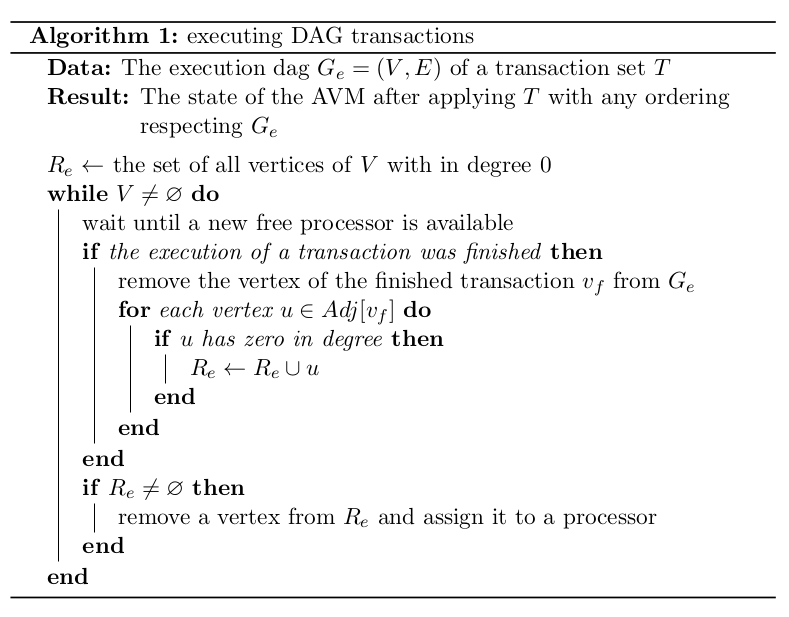
\includegraphics[width=17cm]{../img/Alg1s.png}
\begin{algorithm}
    \DontPrintSemicolon
    \SetKwData{Ready}{$R_e$}\SetKwData{V}{$v_f$}\SetKwData{Graph}{$G_e$}\SetKwData{Vertices}{$V$}\SetKwData
    {Txns}{$T$}
    \SetKwInOut{Input}{input}\SetKwInOut{Output}{output}
    \Input{A sequence of $n$ digits in base $\beta$: $d_{1}d_{2}\dots d_{n}$ \newline
    A prefix tree: $<A^{(1)},A^{(2)},A^{(3)},\dots>$}
    \Output{Valid identifier prefix of the sequence.}
    \BlankLine
    \For{$i = 1$ \KwTo $n$}
    {
        \If{$(0.d_{1}d_{2}\dots d_{i})_\beta < A^{(i)}$}
        {
            \KwRet{$d_{1}d_{2}\dots d_{i}$}\;
        }
    }
    \KwRet{NIL}\;
    \caption{Finding a prefixed identifier}\label{alg:prefix_id}
\end{algorithm}

In Argennon the shorter prefix codes are assigned to more active accounts and smart contracts which tend to own more
data objects in the system. The prefix trees are designed by analyzing empirical data to make sure the number
of leaves in each level is chosen appropriately.


\section{Arithmetics}\label{sec:arithmetics}

The Argennon Virtual Machine supports signed integer and signed floating point operations. The Argennon Virtual
Machine does not support any type of unsigned arithmetics. All arithmetic operations in the Argennon Virtual Machine
are checked and any type of overflow or underflow will cause a catchable exception to be thrown.

\section{Architecture}\label{sec:arch}


\subsection{The \texttt{pc} Register}\label{subsec:the-pc-register}

The Argennon Virtual Machine always has a single thread of execution and exactly has one \texttt{pc} register.
When the Argennon Virtual Machine is executing a method, if that method is not native, the \texttt{pc} register
contains the address of the AVM instruction currently being executed. If the method currently being executed
is native, the value of the Argennon Virtual Machine's \texttt{pc} register is undefined.

\subsection{Call Stack Queue}\label{subsec:call-stack}

Every AVM execution session has a queue of call stacks. A call stack contains all the information that is needed for
restoring the state, and continuing the execution after the method invocation completes.
This information is represented by a \texttt{CallInfo} struct:
\begin{verbatim}
CallInfo {
    applicationID,
    methodID,
    pc,
    canModify,
    localFrame,
    operandStack
}
\end{verbatim}
The \texttt{applicationID} field is the unique identifier that the AVM assigns to every smart contract,
\texttt{methodID} is the unique identifier of a method's bytecode and \texttt{canModify} is a flag
indicating whether a method is allowed to execute state modifying instructions or not.

Every method invocation has a corresponding \texttt{CallInfo} struct and when a method is invoked its
\texttt{CallInfo} struct is pushed onto the call stack. Hence, the top of the call stack always contains
the \texttt{CallInfo} struct of the current method. When a method invocation completes its call
information is popped from the call stack.

An AVM execution session will continue as long as there is a non-empty call stack in the call stack queue. When the
execution of the current call stack finishes the execution of the next call stack in the call stack queue starts.
It's possible that an AVM method invocation creates new call stacks. These newly created call stacks will be a part
of the current execution session and are added at the end of the call stack queue. A newly created call stack always
contains a single \texttt{CallInfo} struct. See Section~\ref{subsec:method-invocation} for more details.

\subsection{Run-Time Data Areas}\label{subsec:data-areas}

The Argennon Virtual Machine defines various run-time data areas that are used during an execution session
(i.e.\ transaction), Some of these data areas are persistent and are stored on the blockchain, Other data areas
are per execution session or per method invocation. These data areas are created when their context starts and
destroyed when their context ends.

The Argennon Virtual Machine has five run-time data areas:
\begin{itemize}
    \item Method Area
    \item Constant Area
    \item Local Frame
    \item Operand Stack
    \item Heap
\end{itemize}
All data areas except operand stack, have their own address space. Operand stack is a
last-in-first-out (LIFO) stack and is not addressable. Every AVM instruction operates on its specific
data areas.

\subsubsection{Method Area}

The method area contains the byte-code of any method which can be called by a non-native method invocation
instruction. In the Argennon Virtual Machine every method has a unique identifier:
\texttt{methodID}, and the method area is a map from method identifiers to their byte codes.

Instructions that modify the code area can only be run in privileged mode which means they can only be executed
by the \emph{root} smart contract. As a result, the access of smart contracts to the code area is essentially
read-only.

\subsubsection{Constant Area}

Every smart contract has a single constant area which is stored in the AVM code area as a special type of
non-executable method. The constant area of a smart contract contains several kinds of constants, ranging from user
defined constants to method address tables. A method address table stores the list of methods of a smart
contract and their access type. The access type of method can be either \texttt{external} or \texttt{internal}.
Only external methods can be invoked by \texttt{invoke\_external} instruction.

\note{Instructions that modify the constant area can only be run in privileged mode.}


\subsubsection{Local Frame}

A local frame is used to store methods parameters and local variables. A new frame is created each time a method
is invoked, and it is destroyed when its method invocation completes, whether the completion is normal or abrupt.

\subsubsection{Operand Stack}

Every time a local frame is created, a corresponding empty last-in-first-out (LIFO) stack is created too. The
Argennon Virtual Machine is a stack machine and its instructions take operands from the operand stack, operate on
them, and push the result back onto the operand stack. An operand stack is destroyed when its owner method
completes, whether that completion is normal or abrupt.

\subsubsection{Heap}

The heap of the Argennon Virtual Machine is a persistent memory area which stores \emph{memory chunks}. A Memory
chunk is a byte addressable piece of continuous memory which has a separate address space starting from 0. Each chunk
has a fixed size and different chunks need not be equally sized. Chunks are stored in the heap area and every chunk is
assigned a unique identifier: \texttt{chunkID}. As a result, the address of every memory location inside
the heap area can be considered as a pair: \texttt{(chunkID, offset)}.

A smart contract can read any chunk stored in the heap by having its \texttt{chunkID}. However, it can only modify
those chunks that was created by itself. In other words, every memory chunk in the AVM heap has an owner. Only
the owner can modify a chunk while anyone can read that chunk. In addition, for modifying a chunk the \texttt{canModify}
flag of the current method's \texttt{callInfo} struct must be true. The owner of a chunk can be easily determined
by the \texttt{applicationID} part of the chunk identifier.

\note{The reason behind this type of access control design is the fact that smart contract code is usually
immutable. That means if a smart contract does not implement a getter mechanism for some parts of its internal
data, this functionality can never be added later. Although the internal data is publicly available, there will
be no way for other smart contracts to use this data on-chain. This design eliminates the need for implementing
\emph{trivial} getters.}

The AVM Heap is able to save snapshots of its state and later restore them. This will enable the Argennon
Virtual Machine to have state reversion capability. The snapshot management of the heap area is done by
the following functions:
\begin{itemize}
    \item \texttt{Save()} saves a snapshot of the current state of the heap and pushes it onto the
    snapshot stack.
    \item \texttt{Restore()} pops the snapshot stored on the top of the snapshot stack and restores it. The
    current state of the heap will be lost.
    \item \texttt{Discard()} pops the snapshot stored on the top of the snapshot stack and discards it. The current
    state of the heap will not change.
\end{itemize}

\note{These functions are internal functions of the AVM. They are not instructions, and can not be called by smart
contracts.}

\section{Instruction Set Overview}\label{sec:instruction-set-overview}

An Argennon Virtual Machine instruction consists of a \textbf{one-byte} opcode specifying the operation to be
performed, followed by zero or more operands supplying arguments or data that are used by the operation.
The number and size of the operands are determined solely by the opcode.

\subsection{Method Invocation}\label{subsec:method-invocation}

The Argennon Virtual Machine has four types of method invocation instruction:
\begin{itemize}
    \item \texttt{invoke\_internal}: invokes a method without changing the context of method execution. In other
    words, \texttt{applicationID} and \texttt{canModify} fields of the invoked method in the
    call stack will be the same as the invoker.
    A smart contract can invoke any method by \texttt{invoke\_internal} instruction, even if that method is an
    internal method of another smart contract. Since the invoked method will always be executed in the context of
    the invoking smart contract, a smart contract will not be able to modify another smart contract state by
    this instruction. This instruction facilitates code reuse and the usage of libraries.
    \item \texttt{invoke\_external}: invokes a method and changes the context of method execution to another
    smart contract. Only external methods of another smart contract can be called by this instruction. For changing
    the context of method execution this instruction sets the \texttt{applicationID} field of the invoked method
    to the \texttt{applicationID} of the called smart contract. Then it searches the call stack and if
    the \texttt{applicationID} of the called smart contract is found in the current call stack it sets
    \texttt{canModify} to \texttt{false}, otherwise \texttt{canModify} is set to \texttt{true}.
    As a result, if the called smart contract is already called, the invoked method will not be
    able to modify the heap area.
    \item \texttt{invoke\_native}: invokes a method that is not hosted by the Argennon Virtual Machine. By this
    instruction, high performance native methods of the hosting machine could become available to AVM smart
    contracts. This instruction will not modify the AVM state.
    \item \texttt{spawn}: spawns a new method invocation. Spawning a method invocation is the invocation of a method
    with changing the context of method execution and creating a new call stack. Only external methods can
    be spawned. The created call stack is added at the end of the call stack queue and
    the \texttt{canModify} field of the pushed \texttt{CallInfo} struct will always
    be set to \texttt{true}. This instruction does not modify the \texttt{pc} register and the execution of the
    caller will continue after this instruction. As a result, \texttt{spawn} can not return
    any value to the caller and the return value of the called method (if any) will be added
    to the transaction output. If the invoked method completes abruptly, it will cause all the call stack queue to
    complete abruptly.
\end{itemize}

\note{The AVM does not natively support polymorphism and virtual methods. A compiler could easily
generates appropriate code for implementing these features.}

Each time a method is invoked the \texttt{Save()} function of the AVM heap is called, then a new local frame
and operand stack is created. The Argennon Virtual Machine uses local frames to pass parameters on
method invocation. On method invocation, any parameters are passed in consecutive local variables stored in the
method's local frame starting from address 0. The invoker of a method writes the parameters in the local frame
of the invoked method using \texttt{arg} instructions.

\note{For AVM smart contracts \emph{reentrancy} can only happen in read-only mode and is totally safe.
At the same time, call-back patterns can be easily implemented by using \texttt{spawn} instruction.}

\subsection{Exceptions}\label{subsec:exceptions}

An exception is thrown programmatically using the \texttt{athrow} instruction. Exceptions can also be thrown by
various Argennon Virtual Machine instructions if they detect an abnormal condition. Some exceptions are not
catchable and will always abort the method invocation.

\note{By using the \texttt{athrow} instruction properly, a programmer can make any method act like an atomic
operation.}

\subsection{Method Invocation Completion}\label{subsec:method-invocation-completion}

A method invocation completes normally if that invocation does not cause an exception to be thrown, either
directly from the AVM or as a result of executing an explicit throw statement. If the invocation of the current
method completes normally and the invocation was made by an \texttt{invoke} instruction, then a value may be
returned to the invoking method. This occurs when the invoked method executes one of the return instructions, the
choice of which must be appropriate for the type of the value being returned (if any). Execution then continues
normally in the invoking method's local frame with the returned
value (if any) pushed onto the operand stack. If the method was invoked by a \texttt{spawn} instruction,
the execution of the next call stack (if any) begins and the returned value
is appended at the end of the transaction output. When a method invocation completes normally,
the \texttt{Heap.Discard()} function is called as a part of the return instruction.

A method invocation completes abruptly if an exception is thrown and is not caught by the current method. A
method invocation that completes abruptly never returns a value.

When a method completes, whether normally or abruptly, the call stack is used to restore the state of the invoker,
including its local frame and operand stack, with the \texttt{pc} register appropriately restored and incremented
to skip past the method invocation instruction. If the current call stack is empty the next call stack in the call
stack queue will be used for continuing the execution, and when there are no call stacks left in the queue the
current execution session ends.

A thrown exception causes methods in the call stack to complete \emph{abruptly} one by one, as long as the
\texttt{pc} register is not pointing to a \texttt{catch} instruction. The \texttt{catch} instruction acts like a
branch instruction that branches only if an exception is caught. When an exception is thrown
Algorithm~\ref{alg:Abrupt} is used to restore the state of the AVM heap.

\begin{algorithm}
    \DontPrintSemicolon
    \SetKwData{Heap}{Heap}\SetKwData{Stack}{CallStack}
    \SetKwFunction{Discard}{Discard}\SetKwFunction{Pop}{pop}\SetKwFunction{Restore}{Restore}
    \SetKwProg{Fn}{Function}{}{}

    \While{\Stack is not empty}
    {
        \Stack.\Pop{}\;
        \eIf{\Stack is not empty \textbf{and} $\Stack[head].pc \rightarrow catch$}
        {
            \Heap.\Restore{}\;
        }{
            \Heap.\Discard{}\;
        }
    }
    \Heap.\Restore{}\;
    \caption{Abrupt method completion}\label{alg:Abrupt}
\end{algorithm}

A closer investigation of Algorithm~\ref{alg:Abrupt} shows that when an invocation which was made by
a \texttt{spawn} instruction completes abruptly, the heap snapshot that was saved before the start of the
execution of the first call stack of the execution session is restored. Since the root
smart contract calls \texttt{Heap.Save()} function before spawning the requested method, this means
that all changes made to the AVM heap during the execution session will be restored, but the changes made by
the root smart contract including the transferring of the transaction fee will not be restored. See
Section~\ref{sec:execution-sessions} for more details.


\subsection{Heap Allocation and Deallocation}\label{subsec:heap-allocation-instructions}

Heap allocation and deallocation in the Argennon Virtual Machine is done by the following instructions:

\begin{itemize}
    \item \texttt{alloc}: creates a new memory chunk of the specifies size in the heap. the identifier
    of the new chunk will be the concatenation of the \texttt{applicationID} of the creator of the chunk and
    the \texttt{id} operand. The specified identifier must be concatenation of
    an \texttt{accountID} and a prefix code
    generated by the \emph{local} prefix tree: \texttt{id = accountID|localID}. If the identifier is not valid or
    if it already exists in the heap a catchable exception will be thrown.

    \item \texttt{delete}: deletes the chunk that its identifier is the concatenation of the current smart
    contract \texttt{applicationID} to the specified \texttt{id}. If the identifier is not valid or
    if the chunk was not found a catchable exception will be thrown.
\end{itemize}

When a smart contract allocates a new memory chunk, the identifier of the new chunk is not generated by
the AVM, instead the smart contract can choose an identifier itself. This is a very important feature of
the AVM heap which allows smart contracts to use the AVM heap as a dictionary (map) data structure.
Because the \texttt{chunkID} is a prefix code, any smart contract has its own identifier space and a smart contract
can easily generate unique identifiers for its chunks.

The AVM requires the chosen identifier to be a prefix code made by concatenating a code compatible with
the \emph{accounts} prefix tree to a code compatible with the \emph{local} prefix tree. This requirement will
enable AVM to detect invalid identifiers while smart contracts can easily associate data with account identifiers.
At the same time, A smart contract is able to create maps with costume keys by appending local identifiers
to the \texttt{accountID} zero, which does not correspond to a valid account in the Argennon.


\section{Execution Sessions}\label{sec:execution-sessions}

The execution of smart contracts code in the AVM is done in execution sessions. Every execution session in the
Argennon Virtual Machine consists of a single method invocation from the \emph{root} smart contract and a list
of resource allocation requests. These allocation requests always include a request for allocating some amount
of execution time and a request for accessing some memory locations for reading or writing. If after the start
an execution session tries to violate its allocated resources, an \textbf{uncatchable} exception will
be thrown by the AVM\@.

\note{The AVM does not have a \texttt{calldata} memory area. The arguments of the root smart contract method will
be copied from the transaction to the local frame of the invoked method, exactly like a normal method invocation.}

The root smart contract with the \texttt{applicationID} of zero, is a special smart contract in the Argennon
Virtual Machine. Its code is immutable and is a part of the AVM implementation. The root smart contract is always
run in the privileged mode, and every execution session starts with a call to a method of the root smart contract.
This method always transfers some amount of fee from an account ot the \texttt{feeSink} account and then it
performs the requested operation.

\note{Argennon transactions do not have a sender, and the payer of the transaction fee could be any
account who has provided the required digital signature.}

If the requested operation is a method invocation, the root smart contract will call the \texttt{Heap.Save()}
function once, and then it will invoke the requested method using \texttt{spawn} instruction. This means that the
invoked method will have a separate call stack and if it completes abruptly the changes made by the root
smart contract to the state will not be reverted.


\section{Authorizing Operations}\label{sec:authorizing-operations}

In blockchain applications, we usually need to authorize certain operations. For example, for sending an asset
from a user to another user, first we need to make sure that the sender has authorized this operation. The
Argennon virtual machine has no built-in mechanism for authorizing operations, but it provides a rich set of
cryptographic instructions for validating signatures and cryptographic entities. By using these instructions and
passing cryptographic signatures as parameters to methods, a programmer can implement the required logic
for authorizing any operation.

\note{The Argennon virtual machine has no instructions for issuing cryptographic signatures.}

In addition to signatures, a method can verify its invoker by using \texttt{get\_parent} instruction. This
instruction gets the \texttt{applicationID} of the smart contract that is one level deeper than the current
smart contract in the call stack or if there is none, the smart contract that created the current call stack.
In other words, it returns the \texttt{applicationID} of the smart contract that has invoked or spawned
the current smart contract.


\section{The AVM Standard Library}\label{sec:the-avm-standard-library}
